\documentclass[12pt]{article}
\usepackage{MinionPro}
\usepackage{CJK}
\usepackage{indentfirst}
\usepackage{graphicx}
\begin{document}
\begin{CJK}{UTF8}{cwmb}

\title{低利率是否造就高房價?}
\author{劉彥佑 (R99628130)\\
李卿澄 (B97501046)\\
黃博億 (B99101014)\\
王祉婷 (B00704056)}
\date{\today}


\maketitle

\section{低利率環境}

今週刊「揭開央行賺錢神話」\footnote{http://mag.chinatimes.com/mag-cnt.aspx?artid=11806\&page=1}一文中提及,我國中央銀行維持或增加其營收的方法不外乎多賺一點與少花一點。多賺一點,也就是增加收入的部份,是透過盡可能累積外匯存底,增加利息收入;而少花一點,則是壓低利率,阻升新台幣匯率。我國中央銀行的獲益主要受到了外匯存底總量、國外利率環境、定存單總量、定存單利率與新台幣匯率五項因素所影響,而除了國外的利率環境央行沒有辦法控制之外,剩下的四項央行都有一定的控制力。\\

為了增加央行的收入,央行要釋出更多的新台幣購買外匯,使外匯存底增加,這樣外匯的利息收入就會增加,而定存單的總量不能多,央行發行的的定存單的利率偏低,以及為了阻升新台幣匯率等為了減少支出且增加收入的作法,將會使得市場上有更多的新台幣。\\

當市場上的新台幣過份充裕時,可貸資金市場的可貸資金增加,為了把錢貸出去以使可貸資金市場重新回到供需平衡點,利率便會降低。假設我國中央銀行以獲利為目的時,中央銀行的操作將使得利率降低,事實上,自2000年後我國的名目利率變大幅度的降低至約2\%的水準,大部分的時間甚至是更低,已經進入了長期低利率的時代。

\section{實質負利率不賺反虧}

透過費雪公式,我們知道實質利率大約等於名目利率減去通貨膨脹率。我們將中華郵政一年期定存的利率作為名目利率,利用主計處公佈的的消費者物價指數來計算通貨膨脹率,將名目利率減去通貨膨脹率來估計近年來我國的實質利率。\\

\begin{figure}[htp]
\centering
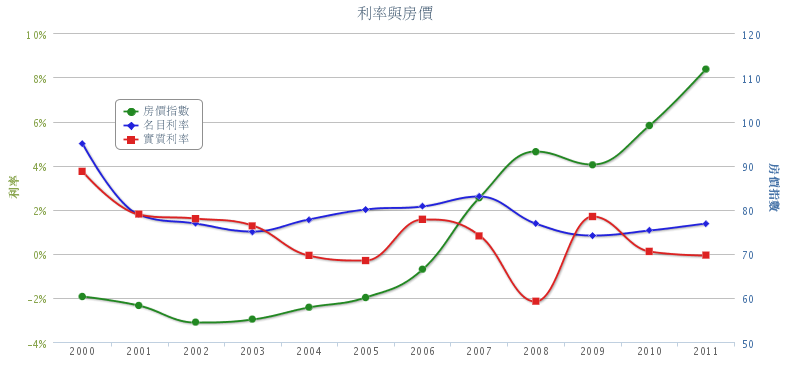
\includegraphics[scale=0.45]{01.png}
\caption{利率與房價}
\label{}
\end{figure}

由圖1可以發現,自西元2001年起,我國的實質利率就沒有高過2\%,甚至在西元2004年至西元2005年以及西元2007年至西元2009年間是負值,在西元2008年出現最低的利率約為-2\%。\\

實質負利率代表了什麼?代表了物價上漲的幅度已經超過了新台幣孳息的幅度。雖然把錢存在銀行中,名目利率雖然是正值,錢的數字會不斷的變大,但雖著時間推移,購買貨品的能力卻沒有成長,反而還下降,換句話說,就是錢竟然越存越小了。把錢存放在銀行不僅不能賺錢,而且還會虧錢!我們相信,人們發現、知道這個事實後,絕對不會放任自己的資產縮水,人們必須找到一個方法或管道,盡可能地不要使資產縮水,這也就是該文中提到的「衝擊四:賺不到利息 全民競逐高風險資產」。

\section{房貸利率下降活絡房市需求}

房地產的價格相較於普通的商品,價格算是非常的高昂,大多數的人們購買房屋都需要向銀行借貸,因此,房屋貸款利率的高低也是影響一般家庭固定投資的因素之一。\\

\begin{figure}[htp]
\centering
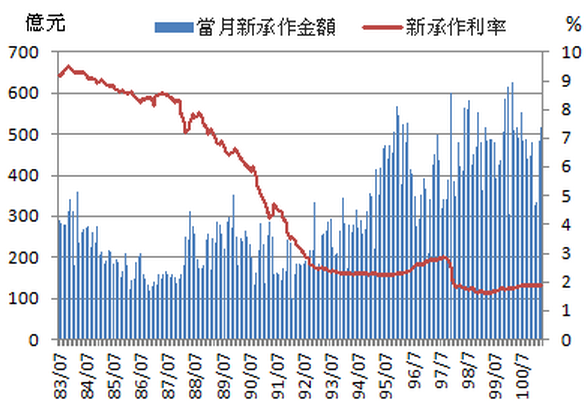
\includegraphics[scale=0.3]{02.png}
\caption{新承作房貸金額與利率(中央銀行)}
\label{}
\end{figure}

西元1995年以後,房貸利率呈現下降趨勢。西元2002年,新承作房貸利率由年初5\%降至年尾3.6\%,對照圖1與圖2,此時房價指數觸底,房地產市場開始回溫。2003年7月以後(至2012年4月),新承作房貸利率維持在1.6\%~3\%之間,新承作房貸金額劇增。2006年以後,各個月份的新承作房貸金額大都維持在300億以上水準,低的房貸利率增加了購屋意願,房價從此高居不下,一飛衝天。

\section{投資需求推升房價走揚}

前面幾段說明了我國處於低利率,甚至實質負利率環境的可能原因。低利率使借貸的成本下降,更多的人願意貸款買房子。此外,低利率也使得存款的報酬率下降,為了防止資產縮水,房地產市場就成為不錯的投資標的。因此,需求增加的結果便是推升了房地產的價格。\\

當既有房屋成交價格攀升時,對於當時的人來說,就有更高的信心認為投資地產已經不僅僅只是為了保有價值,更能夠成為獲利的商品,而且這樣的商品的投資報酬率更勝於將錢存放在銀行中。因此又會有更多的人們願意投資房地產,但供給的增加並不是那麼容易,除了房屋的建設需要長時間之外,以都會區來說,能利用的土地是越來越少。\\

圖1顯示了以2010年為基期的台北市的房地產價格指數。資料取自政府網站「不動產價格e點通」\footnote{http://etp.cpami.gov.tw}。為了瞭解房價與利率的關係,我們將房地產價格指數與實質利率、名目利率一同作比照。\\

由圖1可以發現,自2001年起,名目利率與實質利率一直維持在2\%以下,而房價指數則自2002年以後逐步上升。2007至2008年間,實質利率大幅度的由約1\%下降至-2\%,同時期的房價指數呈現大幅度躍升。隔年實質利率由-2\%回升至2\%左右,相應的房價指數則出現2002年以來唯一一次的大幅度下跌。2009年後,實質利率再度接近0\%,而房價又繼續上漲。\\

\begin{figure}[htp]
\centering
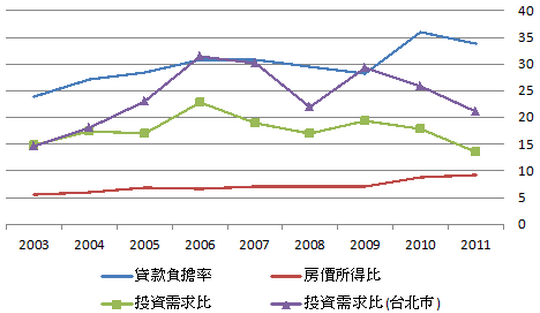
\includegraphics[scale=0.3]{03.png}
\caption{貸款負擔與投資需求(內政部營建署)}
\label{}
\end{figure}

\section{台灣人越來越買不起房子}

圖3是內政部營建署針對台灣五大都會區(台北市、台北縣、桃竹縣市、台中縣市、高雄縣市、台南縣市)的統計資料。圖中顯示2003年以來,台灣五大都會區的房價所得比(30坪中古屋的平均房價/平均年國民可支配所得)不斷創高,2011年已接近10,也就是說平均每個人要不吃不喝十年才能買下一棟房子。\\

很多人會想,利率那麼低,先貸款買個房子總比什麼都沒有來的好。但是在所得沒有增加的情況下,房奴們更是被房貸壓得喘不過氣來。2003年的貸款負擔率(每月房貸支出佔家庭月所得比)為24\%左右,2011年提升至34\%。\\

房價的高居不下,究竟是實質需求的推升,還是投資需求所吹起的泡泡呢?關於這個問題,我們認為有一定的實質需求是存在的。圖3顯示台灣五大都會區的投資需求比(與住宅需求比之總和為100\%,此圖沒畫出住宅需求比)自2003年以來大致上維持在15~20\%的區間內,而台北市的投資需求比,則呈現上升趨勢,大約比五大都會區高了5個百分點。由此可見投資需求可能主要集中於都會的精華區,或是即將開發的地區。\\

綜合前面各節所述,我們認為政府的低(房貸)利率政策並不能根本的解決民眾買不起房的問題,可能還會推升房價走高。政府應該做的是創造更多的就業與投資機會,或許等到均衡利率走升的時候,才是一般老百姓買得起房的時候吧!

\end{CJK}
\end{document}
